Afin de répondre à l'aspect "boîte noire" des réseaux de neurones, nous avons implémenté une interprétabilité dans notre modèle à l'aide de Grad-CAM~\cite{GRADCAM}. Cette méthode permet de fournir une explication visuelle vis-à-vis des décisions de classification issue de notre modèle, permettant ainsi de rajouter une certaine légitimité relative face à nos analyses de traces de sang faisant partie d'un processus judiciaire. 

\subsection{Visualisation avec Grad-CAM}
L'algorithme Grad-CAM (Gradient-weighted Class Activation Mapping) est une technique utilisée pour rendre les réseaux de neurones convolutifs (CNN) plus interprétables dans le domaine de la classification.
Il fonctionne en générant des cartes de chaleur (heatmaps) qui mettent en évidence les zones importantes d'une image qui contribuent le plus à la prédiction d'une classe spécifique.
Pour ce faire, Grad-CAM calcule les dérivées des scores de sortie de la classe cible par rapport aux caractéristiques de la dernière couche convolutive du CNN.
Ces dérivées sont ensuite globalement moyennées pour obtenir les poids d'importance de chaque carte de caractéristiques.
Enfin, les cartes de caractéristiques sont pondérées par les poids d'importance et combinées pour obtenir la carte de chaleur Grad-CAM, qui peut être superposée à l'image d'origine pour une visualisation plus intuitive.
Cette approche permet de mieux comprendre les décisions prises par le CNN et d'améliorer la confiance dans les prédictions du modèle.
La Figure~\ref{fig:grad_cam_example} montre un exemple d'une image de trace de sang avec sa carte de chaleur Grad-CAM superposée.

\begin{figure}[ht]
    \centering
    \begin{subfigure}{0.35\linewidth}
        \centering
        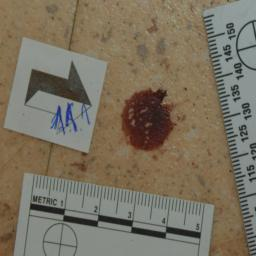
\includegraphics[width=\linewidth]{../asset/exemple/14.jpg}
    \end{subfigure}
    \begin{subfigure}{0.35\linewidth}
        \centering
        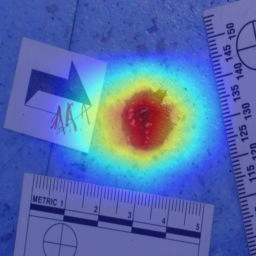
\includegraphics[width=\linewidth]{../asset/exemple/14_saliency.png}
    \end{subfigure}
    \caption{Exemple d'une image  de trace de sang (à gauche) avec sa carte de chaleur Grad CAM superposée (à droite).}
    \label{fig:grad_cam_example}
\end{figure}

En utilisant Grad-CAM, nous avons pu identifier que le modèle se focalisait parfois sur ces réglettes pour prendre sa décision, ce qui nous a permis de mieux comprendre les erreurs de classification, comme le montre la Figure~\ref{fig:grad_cam reglette}.

\begin{figure}[ht]
    \centering
    \begin{subfigure}{0.35\linewidth}
        \centering
        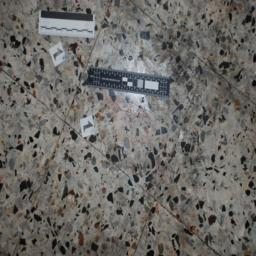
\includegraphics[width=\linewidth]{../asset/exemple/attention_reglette_image.jpg}
    \end{subfigure}
    \begin{subfigure}{0.35\linewidth}
        \centering
        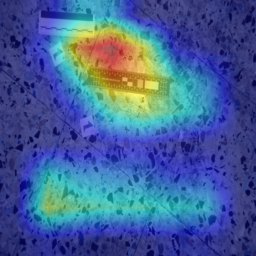
\includegraphics[width=\linewidth]{../asset/exemple/attention_reglette.jpg}
    \end{subfigure}
    \caption{Exemple d'une image de trace de sang (à droite) avec sa carte de chaleur Grad CAM superposée (à gauche), dans le cadre d'une attention portée à la réglette.}
    \label{fig:grad_cam reglette}
\end{figure}

\subsection{Métriques de saliency maps}
De plus, nous avons également implémenté les métriques Average Drop, Average Increase et Average Gain~\cite{opticam}, qui consiste à multiplier l'image de départ par la carte de saillence obtenue avec Grad-CAM puis de redonner cette image au modèle pour obtenir une nouvelle prédiction. On va alors comparer le changement de probabilité de la classe prédite avant et après le masquage de l'image. Ces métriques permettent de quantifier l'exactitude des cartes de saillance obtenues. La section~\ref{sec: grad metrics} présente les formules permettant de les calculer.

L'Average Drop (AD) quantifie la perte de pouvoir prédictif, mesurée en termes de probabilité de classe, lorsque nous masquons uniquement l'image. Elle est comprise entre 0 et 100, et une valeur plus faible est meilleure.

L'Average increase (AI) également connu sous le nom d'increase in confidence, mesure le pourcentage d'images pour lesquelles l'image masquée donne une probabilité de classe plus élevée que l'image originale. Elle est comprise en 0 et 100, et une valeur plus haute est la meilleure.

L'Average Gain (AG) quantifie le pouvoir prédictif, mesuré en tant que probabilité de classe, lorsque nous masquons l'image. Elle est comprise entre 0 et 100, et une valeur plus élevée est meilleure.

La Table~\ref{tab:saliency_results} montre les scores de ses métriques sur la base de données de test des données réelles\footnote{On a effectuer les tests seulement sur les modèles AWL ResNet car c'est les seules dont les poids des couches de convolution ont été appris}.

\begin{table}[ht]
    \centering
    \begin{tabular}{cccc}
        \toprule
        Métriques & Average Drop & Average Increase & Average Gain \\
        \midrule
        AWL ResNet & 91.6 & 0.0& 0.0\\
        FT AWL ResNet & 87.6 & 0.0 & 0.0\\
        \bottomrule
        \end{tabular}
    \caption{Résultats des métriques sur les données réelles (de la base de données de test).}
    \label{tab:saliency_results}
\end{table}

On peut voir dans la Table~\ref{tab:saliency_results} des résultats très peu satisfaisant. En effet, les deux modèles ont une Average Increase et une Average Gain de 0, ce qui signifie qu'avec les notations de la section~\ref{sec: grad metrics}, on a toujours $\forall i \in [1, N], p_i < o_i$. Cela signifie qu'en multipliant l'image d'origine par la carte de saillance, on obtient toujours une probabilité de classe plus faible que l'image d'origine. Cela montre que ces cartes de saillance ne sont pas fiables. Une amélioration possible serait d'utiliser des méthodes de saliency maps plus performantes comme Grad-CAM++~\cite{gradcam++} ou Score-CAM~\cite{scorecam}.
